\documentclass[10pt,letterpaper]{article}
\usepackage{amsmath}
\usepackage{amsfonts}
\usepackage{amssymb}
\usepackage[english]{babel}
\usepackage{breakurl}
\usepackage[superscript]{cite}
% \usepackage{draftwatermark}
\usepackage{fancyhdr}
\usepackage{float}
\usepackage[margin=1in]{geometry}
\usepackage{graphicx}
\usepackage{hyperref}
\usepackage[utf8]{inputenc}
\usepackage{makeidx}
\usepackage{multicol}
\usepackage{nth}
% \usepackage[default,scale=1.0]{opensans}
\usepackage{setspace}
\usepackage{siunitx}
\usepackage{svg}
\usepackage{subcaption}
\usepackage{tikz}
\usepackage{url}
\usepackage{kantlipsum}

%% Preamble
% Custom commands
\newcommand{\ts}{\textsubscript}

% Use hyphans to break up urls
\def\UrlBreaks{\do\/\do-}

% Draft watermark
% \SetWatermarkText{\textsc{Draft}}
% \SetWatermarkScale{5}

% PDF and href setup
% Hyper ref
\hypersetup{
	colorlinks=true,
	citecolor=black,
	linkcolor=black,
	filecolor=black,
	urlcolor=blue,
	pdftitle={Engineering Economic Analysis Report of Renewable Technologies},
	bookmarks=true
}
\urlstyle{same}

% Page semantics
\pagestyle{fancy}
\fancyhead[L]{\slshape\MakeUppercase{MECH 431}}
\fancyhead[R]{\slshape Muchen He}
\fancyfoot{}
\fancyfoot[C]{\thepage}

\parindent 0ex

% Meta
\author{Muchen He}
\title{Renewable Energy For Average Household in Edmonton}
\begin{document}
\begin{titlepage}
	\begin{center}
		\vspace*{3in}
		\line(1, 0){400}\\
		\Huge{\textbf{Renewable Energy For An Average Household in Edmonton}}\\[0.2cm]
		\large{\textbf{Engineering Economic Analysis Report of Renewable Technologies}}\\[1cm]
		\Large{\textbf{MECH 431}}\\
		\textbf{University of British Columbia}\\
		\line(1, 0){400}\\
		\vfill
		\Large{Muchen He}\\
		44638154\\

		\today\\
	\end{center}
\end{titlepage}

% Executive Summary
\section*{Summary}
The renewable energy projects are increasingly becoming attractive. This report explores three options with different scale, and compare it with the cashflow analysis of not doing anything. The electricity rate increases with time and any of the three solutions is better in the long run (after 26 years). However, the alternative with the greatest power output has the least \$ per wattage cost, and thus has the greatest rate of return. Therefore the large scale alternative should be chosen.\\
\clearpage

% Table of contents
\setcounter{secnumdepth}{3}
\tableofcontents
\thispagestyle{empty}
\clearpage

% Uncomment for list of tables and figures
\thispagestyle{empty}
\listoffigures
\listoftables
\newpage

% Set page and section counter
\setcounter{page}{1}

\section{Introduction}\label{section:introduction}

\subsection{Problem}

Edmonton, being the "Oil city", the captial of the province whose major export is oil, is relying too much on non-renewanle resources like fossil fuel. Thus we need to take steps to move towards greener solutions.\\

Edmonton average household consumes an average of between 7500 to 8500 kWh per year. It would be world changing if all these electrical energy can be derived from renewable sources. With the rising prices of means to produce energy, the renewable approach could be economically viable.\\
\\
Alberta consumes more than 10,000 GWh of energy a year. This averages to about 2400 kWh per capita\cite{average-albertan-consumption}. The province has an over-reliance on non-renewable resources for its power generation. Furthermore, projects involving building pipelines and method of hydraulic fracturing (fracking) poses serious environmental impact\cite{fracking-kurzgesagt}.\\
\\
This report intends to explore the economic viablility of renewable solutions that an individual or a family can realistically implement.\\
\\

\subsection{Solution Overview}

To solve this problem, we will look at the economic analysis of solar solutions. The analysis outlines the economic criteria and economic viability of implementing solar generation for a single average household in the sub-urban neighbourhoods of Edmonton.\\
\\
An adequate sustainable solar system should take pressure off of drawing energy from the grid, the electric companies, whose energy is generated from natural gas, coal, and oil. The main parts to a solar system consists of three components\cite{components}:

\begin{enumerate}
	\item Generation: this includes the solar (or commonly referred to as PV) cells that converts photon energy from the sun into electrical voltages. In the context of analsis and design, this would also include the infrastructure setup for these cells, such as mechanical mounting racks, and installation efforts.
	\item Storage: this includes the necessary electrical equipment to ensure extra energy generated from the PV panels could be stored to be used or sold. 
	\item Utilization: this includes the delivery of energy, which consists of equipment to convert generated direct currents (DC) to household appliance compatible alternating current (AC), like an inverter. This component also considers metering the power output such that excess energy can be sold.
\end{enumerate}

\section{Design}

A template will be built from an average house loacted in Edmonton suburban area, I will use my house as a referece. The type of landscape and architecture is ubiquitous throughout Edmonton neighbourhood and thus would make the model adequate.\\
\\
The power analysis and simulation will be based off of this template.\\
\\

\begin{figure}[H]
	\centering
	
\includegraphics[width=0.9\textwidth]{assets/1534567367296}
	\caption{Map of the template house and its relative layout to the neighbourhood}
	\label{fig:template-house-path}
\end{figure}

\subsection{Requirements}\label{requriements}

The requirement is the criteria that determines if the project is a success or fail. The alternatives and layouts we consider should all meet the requirements.\\

\subsubsection{Power Demand}

The average Canadian household consumes 11,135 kWh of electricity in 2014\cite{residential-energy-use}. While Alberta household average is actually lower than the national average: at 7200 kWh. For the sake of analysis and providing a conservative estimate, we will use 8300 kWh per household.\cite{aeso-load-data, ieso-power-data, callmepower}\\

Finding the daily average, the daily energy use is given by

$$
E_\text{daily}=8300\div 365.25 = 22.7\text{kWh per day}
$$

An ideal sustainable system would need to supply at least 22.7 kWh a day on average for everyday of the year. However, we will see later in section \ref{subsection:consumption} that the power demand is non-uniform. On top of that, during winter times, the solar performance is hindered by the reduced hours of sunlight and snow coverage. Having big enough batteries to compensate the reduced generation for an entire season is inconceivable. This issue will be explored in more detail in the weather and generation section \ref{subsection:weather}\\

\subsubsection{Rate of Return}

Because this is an economic analyis of a project meant to save costs in the long-run, we will assume an after-tax MARR of 3\%. This aligns with historical data from the industry.\\

\section{Scenario}\label{scenario}

For this economic analyis, the following assumptions will be asserted. These assumptions are based off of real data.\\
\\
We will assume the solar system is installed for a residential household. Despite that, to incorporate the tax and asset analysis element in this exploration, we will treat the saved costs as operational income. The equipment will be treated as assets with the correspondant CCA class defined by the Canadian Revenue Agency\cite{cca}. As such, the assets will be depreciated by using the method outlined in the course.\\

\subsection{Energy Consumption}\label{subsection:consumption}

As calculated earlier is the requirements subsection (section \ref{requriements}), the yearly average is 8300 kWh. The monthly average is then 692 kWh and  the daily average is 22.7 kWh. All uniformly spreadout throughout the year. To ensure the analyis is more realistic and accurate, we will tweak the usage such that it follows a cosine curve. The characterisitcs of the this consumption curve is derived from real hourly usage data collected by AESO and IESO.\cite{aeso-load-data, ieso-power-data}\\
\\
I derived a formula for monthly consumption such that the yearly average is still 8300 kWh, but the monthly usage varies due to seasonal applicance usage:

\begin{equation}
	\text{Monthly Consumption}=X\cos\left(\frac{m\pi}{6}\right)+M
	\label{eqn:monthly-consumption}
\end{equation}

Where $X$ is the expected fluctuation in consumption between the seasons. Suppose this is 10\% of monthly 692 kWh usage.\\
\\
Where $m$ is the month in numerical form (1 for January, 5 for May, etc.) and $M$ is the monthly average (692 kWh).\\
\\
The projected consumption by our model for each month is computed using equation \ref{eqn:monthly-consumption} in the table as follows (table \ref{table:consumption-table}, figure \ref{fig:consumption-graph}):

\begin{table}[H]
	\centering
	\begin{tabular}{ |c|c| }
		\hline
		Month & Consumption\\
		\hline
		1 & 751.57 kWh\\
		2 & 726.25 kWh\\
		3 & 691.67 kWh\\
		4 & 657.09 kWh\\
		5 & 631.77 kWh\\
		6 & 622.50 kWh\\
		7 & 631.77 kWh\\
		8 & 657.09 kWh\\
		9 & 691.67 kWh\\
		10 & 726.25 kWh\\
		11 & 751.57 kWh\\
		12 & 760.84 kWh\\
		\hline
		Total & 8300 kWh\\
		\hline
	\end{tabular}
	\caption{Modelled monthly electricity consumption}
	\label{table:consumption-table}
\end{table}

\begin{figure}[H]
	\centering
	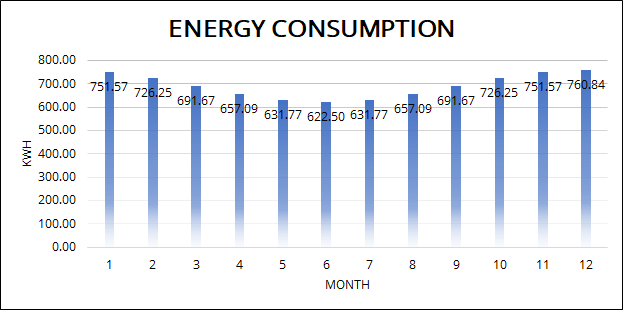
\includegraphics[width=0.7\textwidth]{assets/1534567555536}
	\caption{Modelled monthly electricity consumption (graph)}
	\label{fig:consumption-graph}
\end{figure}

The full detailed calculations can be found in appendix \ref{appendix:consumption}.\\
\\
\subsection{Weather}\label{subsection:weather}

The biggest uncertainty lies in weather. Fortunately, Edmonton is statistically one of the sunniest places in Canada, with 4383 hours of daylight and 2205 of sunlight annually on average\cite{sunshine-canadian,climatemps}.\\
\\
Using this information, we can build a model, similar to that of the monthly consumption to determine the amount of sunlight the PV cells have exposure to.\\
\\
The output is a sinusoid with the peaks at mid-year during summer seasons: (figure \ref{fig:weather-daylight}).\\

\begin{figure}[H]
	\centering
	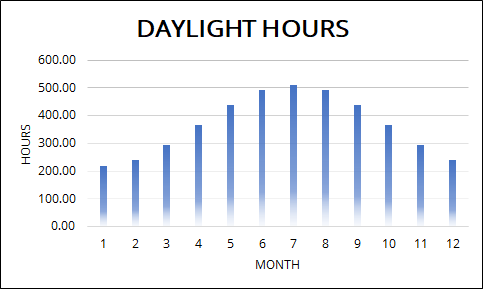
\includegraphics[width=0.6\textwidth]{assets/1534567625830}
	\caption{Model projection of hours of daylight monthly}
	\label{fig:weather-daylight}
\end{figure}

Daylight does not imply direct sunlight. Climatemps concludes that 50.3\% of the daylight time is sunny, 25\% is cloudy or shade, and the rest 24.7\% is other times where sun has low intensity, possibly due to rain, snow, etc\cite{climatemps}. Thus, the number of sunny hours is 50.3\% times the total monthly daylight hours. Likewise for the other two.\\
\\
Now that we classified possible weather to three general states, we can assign a relative solar performance score to each. For sunny weathers, the overall effect on the solar panel performance is minimal, the performance is expected to be at 90\%. This is not 100\% because we need to account for shallow angles of the sun during mornings and evenings. For cloudy, the performance can drop to 50\%, and lastly 25\% performance for overcasts.\\
\\
Using these statistics, we can compute the expected value of the \textit{equivalent hours of direct sunlight} received by the PV cells.

\begin{equation}
	\text{Equivalent hours}=\text{Sunny hours}\times50.3\%+\text{Cloudy hours}\times 25\% + \text{Overcast hours}\times 24.7\%
\end{equation}

We then multiply these equivalent hours by a correction factor such that the projected data will fit better than real collected data from home-owners with solar panels. These data are available from Kuby, a solar systems installation and consulting firm in Alberta\cite{kuby-complete-guide}. The correction factor corrects the loss in efficiency due to more extreme weather conditions in the winter and snow obstructions.\\
\\
The final monthly equivalent sunlight hours is shown in figure \ref{fig:weather-corrected}. This will be directly incorporated into our economic analyis to determine how much grid power we need.\\
\\
\begin{figure}[H]
	\centering
	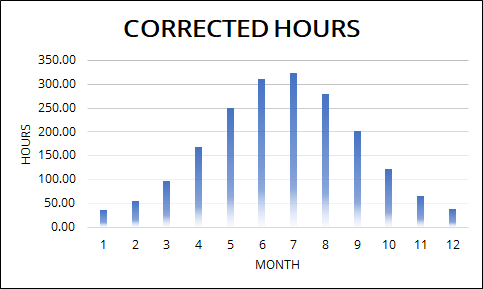
\includegraphics[width=0.6\textwidth]{assets/1534572784062}
	\caption{Corrected equivalent sunlight hours}
	\label{fig:weather-corrected}
\end{figure}

The full detailed calculations can be found in appendix \ref{appendix:weather}.\\
\\

\subsection{Grid Power}\label{subsection:grid}

Using Ontario Energy Board (OEB) collected historical data for time-of-use (TOU) electricity rates as referece, we build a model for the grid power for the next 40 years\cite{oeb}. The collected data goes back to 2006 which should be enough to project a trend. Table \ref{table:grid-history} shows the electricity rates depending on TOU.\\

\begin{table}[H]
	\centering
	\begin{tabular}{|c|c|c|c|}
		\hline
		Year & Off-peak (\$/kWh) & Mid-peak (\$/kWh) &  On-peak (\$/kWh)\\
		\hline
		2006 & \$0.04 & \$0.08 & \$0.11\\
		2007 & \$0.03 & \$0.07 & \$0.09\\
		2008 & \$0.03 & \$0.07 & \$0.09\\
		2009 & \$0.04 & \$0.08 & \$0.09\\
		2010 & \$0.05 & \$0.08 & \$0.10\\
		2011 & \$0.06 & \$0.09 & \$0.11\\
		2012 & \$0.07 & \$0.10 & \$0.12\\
		2013 & \$0.07 & \$0.10 & \$0.12\\
		2014 & \$0.08 & \$0.11 & \$0.14\\
		2015 & \$0.08 & \$0.12 & \$0.16\\
		2016 & \$0.09 & \$0.13 & \$0.18\\
		2017 & \$0.08 & \$0.11 & \$0.16\\
		2018 & \$0.07 & \$0.09 & \$0.13\\
		\hline
	\end{tabular}
	\caption{Historical electricity rates}
	\label{table:grid-history}
\end{table}

Power Stream's data gives into insight into the duration of the peak times. Using that determine for each day, 50\% of the time is off-peak, 25\% of the time is mid-peak and on-peak\cite{powerstreamTOU}. Using this statistics, we find the expected value for electricity each year (equation \ref{eqn:historical-electricity}):\\

\begin{equation}
	\text{EV electricity rates}=50\%\times\text{off-peak rate}+25\%\times \text{mid-peak rate}+25\%\times\text{on-peak rate}
	\label{eqn:historical-electricity}
\end{equation}

Using past electric bills and online sources as references, there are also associated \textit{transmission, distribution}, and \textit{administration} fees associated with each kWh of consumption. Looking at a sample electric bill, the ratio of these fees, relatives to the electricity rates is as follows (table \ref{table:grid-fees}). Note that this only applies to year 2018, as projected rate of increase for electricity is different from rate of increase for distribution and transmission.\\

\begin{table}[H]
	\centering
	\begin{tabular}{|c c|}
		\hline
		Transmission&16.80\%\\
		Distribution&13.00\%\\
		Admin&5.00\%\\
		\hline
	\end{tabular}
	\caption{Rates of other electricity fees as a ratio to main electricity rates}
	\label{table:grid-fees}
\end{table}

The total cost per kWh for 2018 is \$0.1165 per kWh.\\
\\
We assume the projected increase in electricity rates is 5.10\% annually, and the projected rate of increase for transmission and distribution is 2.20\% annualy.\cite{transmission-projection} Using the 2018 rates as base rate, we can compute the cost at some future time. Figure \ref{fig:grid-projection} shows tThe estimated trajectory of grid electricity costs. Full calculations and tables can be found in appendix \ref{appendix:grid}.

\begin{figure}[H]
	\centering
	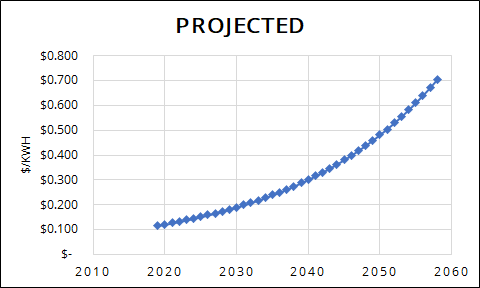
\includegraphics[width=0.6\textwidth]{assets/1534567789488}
	\caption{Projected total cost to electricity per kWh}
	\label{fig:grid-projection}
\end{figure}

According to BCHydro, the current buyback rate for excess generated electricity is 9.99 cents per kWh\cite{bchydro-buyback}, assume a slow but steady growth of 1.0\% a year. The buyback rate could be directly incorporated into our analysis (figure \ref{fig:grid-buyback}).

\begin{figure}[H]
	\centering
	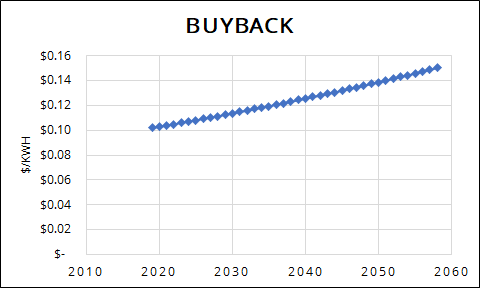
\includegraphics[width=0.6\textwidth]{assets/1534567834603}
	\caption{Projected buyback rate for electricty per kWh}
	\label{fig:grid-buyback}
\end{figure}

\subsection{Government Incentives}\label{subsection:rebate}

Asides from saving money in the long-run and potentiall selling excess energy (see previous section for buyback), the Alberta government and the City of Edmonton offers generous incentives that takes form of a one-time rebate.\cite{kuby-costs,kuby-edmonton,kuby-alberta}\\
\\
The rebate is applied immediately when the project is purchased with cash, or applied immediately and reduces the debt if a loan is taken.\\
\\
Alberta offers a rebate of \$0.75 per W, up to the lesser of \$10,000 or 30\% of the initial cost\cite{kuby-alberta}. The city of Edmonton offers an additional \$0.15 per W, no upper limits.\\

\subsection{Capital}\label{subsection:capital}

There are two main methods of purchasing, cash or loan. For the sake of simplicity, we will assume it is one or the other. We will also assume we have less than \$10,000 of savings immediately in savings. This implies that any setup under the cost of \$10,000 can be paid in cash.\\
\\
Otherwise, we can choose to take a loan. The details for the loan is up to the contractor. This will be specified in the differente alternatives in the alternatives section (section \ref{section:alternatives}).\\
\\
For loans, it is commonly to be relative to a \textit{prime rate}. In this case, we use the recent data from yCharts which shows 3.0\%.\cite{prime-rate} We assume that this rate won't change.\\
\\
Finally, we will use a conservative constant 2\% annual inflation rate based on historical data.\cite{inflation} We assume this rate do not change for the duration of the analysis.\\

\subsection{Depreciation and Taxes}

Since we treat the cost savings as a business income, they will be taxed like a business. The corporation tax for new, small businesses is 10\% according to the Revenue Agency\cite{business-tax}.\\
\\
Any non-contracted purchases will be subject to a local sales tax GST of 5.0\%.\\
\\
Purchases that has a defined CCA class will be added to a UCC account. The book value for that account will be depreciated by the corresponding CCA class rate. In this analysis, we conservatively assume that excess tax credit are not carried on to the next year, and that the government will not provide negative tax (positive cashflow).\\

\subsection{Maintenance and Wear}

The assets in this analysis, mainly the solar panels require cleaning. This falls under the Maintenance fees. Using known data from solar companies, it is estimated to be \$0.01 per W per year of solar panels.\cite{kuby-costs} This cost incorporates the cost of cleaning equipment (water) and opportunity costs (time).\\
\\
Furthermore, the solar panels are known to have its efficiency wear out at a rate of 0.5\% annualy. We assume that this rate do not change and we only install replacements with similar technologies.\\
\\
On top of the 0.5\% wear, the solar panels will, on average, suffer an additional flat 2.0\% efficiency decrease due to dust and soiling on the solar panel surfaces. Hence the \$0.01 per W per year of Maintenance costs.\\

\subsection{Salvage}

At the end of the analysis period, we assume the salvage value to be the left over amount in the depreciable asset's book value.\\
\\

\subsection{Analysis Periods}

We will run the analysis period for three time-scales:

\begin{itemize}
	\item short-term (5 years) - appropriate for if we don't stay at the house very long (such as for when the house gets sold or rented out). Since 5 years is short, it's likely that the equipment and technology are not yet obsolete. Thus for this analysis period, we would account for the extra salvage value / resale value at the end of the 5 year period.\\

	\item medium-term (20 years) - this is the most realistic time period for most home-owners. The projection of power company electricity costs will be estimated using cost-index. The improvement in technlogy for the replaced solar panels are modelled as learning curve model.\\

	\item long-term (40 years) - this analysis period is appropriate for long term residency. The market price, cost index, and technology efficiency would be quite inaccurate in the far future. The assumption is that we would still be using the same system.
\end{itemize}

\section{Alternatives}\label{section:alternatives}

This section outlines the four different main alternatives that we will be exploring.\\

\subsection{Do Nothing}

The "Do nothing" alternative implies nothing is invested into solar energy. There will be no rate of return, savings, or rebates.\\
\\
Note that this will be used as reference for other three alternatives to analyize the relative benefits and savings.\\ 

\subsection{A - Small Scale (0.4 kW)}

The small scale alternative involves a very cheap approach to solar energy. The solution is offered as a kit from retailers such as HomeDepot and amazon.ca\cite{amazon-small, homedepot-small}.\\
\\
For a clearer analysis, I looked up the quantity and costs for the individual parts contained in this kit on their respective websites. The components' belongs to CCA class 8 and depreciation rates of 30\%. Furthermore, everything except for the solar cells is assumed to have a flat lifetime of 10 years (need replacement after 10 years of use). The solar cell will have a replacement analysis of its own.\\
\\
Putting everything together, the parts are as follows in table \ref{table:small-parts-list}:

\begin{table}[H]
	\centering
	\begin{tabular}{|c|c|c|c|}
		\hline
		Part&Qty.&Cost ea. & Depre. Rate \\
		\hline
		100 W PV cells & 4 & \$238.00 & 30\%\\
		Charge controller &1& \$150.00&30\%\\
		Inverter &1& \$539.50&30\%\\
		Battery &8& \$26.00&30\%\\
		\hline
	\end{tabular}
	\caption{Parts list for alternative A}
	\label{table:small-parts-list}
\end{table}

The subtotal of all parts together including the 5.0\% GST is \$1,941.98. The install time is approximately 4 hours with a solar technician. The cost to install is \$24 per hour of labour for a solar technician\cite{solar-technicial-1,solar-technicial-2}. So we add an additional \$96.00 to the initial cost.\\
\\
The total rebate is $(0.15+0.75)\times(400)=360$ dollars. We subtract this value from our initial cost.\\
\\
Finally, our total initial cost is  \$1,677.98. Since we have enough cash on hand (as assumed earlier in subsection \ref{subsection:capital}, we don't need to take a loan on this.\\

\subsection{B - Medium Scale (5 kW)}

This alternative is significantly larger than the previous alternative. Installing, by Alberta law, requires a certified professional installation service. In this case we do not need to consider the cost of individual parts. However, in order to keep track of the depreciable assets, we need to account for the value of the installed parts.\\
\\
Generally, the larger the solar generator, the smaller the investment amount per capacity (W). Kuby, the solar system company reveals that on average, the cost per W for a specified kW system is as follows (figure \ref{fig:cost-per-w}).\cite{kuby-costs} The linear line of best fit shows the linear relationship: $\$=2900(\text{kW})+4120$.

\begin{figure}[H]
	\centering
	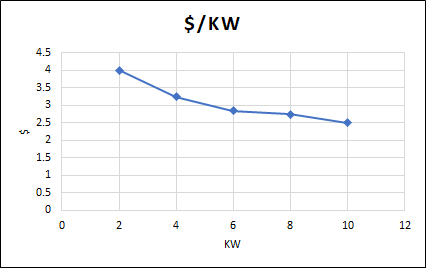
\includegraphics[width=0.6\textwidth]{assets/1534567923498}
	\caption{Cost per W for a system with specific kW capacity}
	\label{fig:cost-per-w}
\end{figure}

Using this relationship, we can determine that our 5 kW system would require a total of \$18,620.00. Using the same rebate calculation (subsection \ref{subsection:rebate}) as before, we determine the rebate value to be \$4,500.00. The initial cost we have to pay is \$14,120.00\\
\\
Even with rebate, the initial cost is too expensive for us to afford using cash. Therefore we have the option to take out a loan with either 5 or 15 year terms with no down payment.\\
\\

The company also shows the breakdown of the cost given some total contracting cost (figure \ref{fig:cost-breakdown}):

\begin{table}[H]
	\centering
	\begin{tabular}{|c|c|}
		\hline
		Type&Fraction of total cost\\
		\hline
		PV panels&35\%\\
		Inverters&20\%\\
		Mechanical&9\%\\
		Electrical&14\%\\
		Planning&4\%\\
		Permitting&2\%\\
		Labor&16\%\\
		\hline
	\end{tabular}
	\caption{Cost breakdown of a typical medium to large sized residential solar system}
	\label{fig:cost-breakdown}
\end{table}

The PV panels and inverters fall under CCA class 43 at a depreciation rate of 30\%. The mechanical components such as mounting, racks, and conduits, fall under CCA class 17 with depreciation rate of 10\%. The electrical parts consists of wiring, batteries, insulation, fall under the CCA class 8, with depreciation rate of 20\%.\\
\\
The planning, permitting, and labor costs are unavoidable as Alberta law requires solar installation of this size to be performed by certified professions, as well as checked by engineers to ensure safety. These costs are not depreciable as they are not spent on assets. Because all these assets depreciate at a different rate, we need to keep three accounts for all assets.\\
\\
The amount for each fraction of the total cost is as follows in figure \ref{fig:medium-cost-breakdown}:\\

\begin{table}[H]
	\centering
	\begin{tabular}{|c|c|}
		\hline
		Type&Fraction of total cost\\
		\hline
		PV panels&\$11,592.00\\
		Inverters&\$6,624.00\\
		Mechanical&\$2,980.00\\
		Electrical&\$4,636.80\\
		Planning&\$1,324.80\\
		Permitting&\$662.40\\
		Labor&\$5,299.00\\
		\hline
	\end{tabular}
	\caption{Broken-down costs for a medium capacity system}
	\label{fig:medium-cost-breakdown}
\end{table}

Note that the inverters and electrical parts, like alternative A, needs to be replaced every 10 years. There are no rebates for replacements.\\
\\

\subsection{C - Large Scale (10 kW)}

This alternative is the same as alternative B, except with higher capacity by deploying more solar panels, having larger batteries, etc. Despite being twice the capacity, the linear relationship used for alternative B still applies. The estimated total cost is $2900(\text{10 kW})+4120$=\$33,120.00.\\
\\
Applying the same rebate conditions, the rebate value is \$9,000.00.\\ The total cost we have to pay is \$24,120.00. Again, we need to choose either 5 or 15 year term loans with no down payment because we cannot to afford via cash.\\

\section{Cashflow Analysis}

\subsection{Do Nothing}

For doing nothing, the power consumed from the grid is a constant 8300 kWh per year. We multiply this by the electricity rates of that year as projected in subsection \ref{subsection:grid}.\\
\\
The energy cost for any particular is given by:

\begin{equation}
	\$=8300\times E_n
\end{equation}

where $E_n$ is the expected value electricity rate for year $n$. Then we take this \textit{real} cost and convert it to nominal cost because of inflation:

\begin{equation}
	\text{\$ nominal}=\frac{\text{\$ real}}{(1+f)^n}
\end{equation}

where $f$ is the inflation rate, 2\%, and $n$ is the year.\\

The result is an increasing nominal yearly cost to electricity (as shown in table \ref{table:cf-nothing-cf} and figure \ref{figure:cf-a}).\\
\\
\begin{table}[H]
	\centering
	\begin{tabular}{|c|c|}
		\hline
		Year&Nominal yearly cost\\
		\hline
		1&\$991.13\\
		2&\$1,015.79\\
		3&\$1,041.20\\
		4&\$1,067.37\\
		5&\$1,094.32\\
		\vdots&\vdots\\
		20&\$1,610.79\\
		\vdots&\vdots\\
		40&\$2,776.13\\
		\hline
	\end{tabular}
	\caption{Nominal cashflow each year for doing nothing}
	\label{table:cf-nothing-cf}
\end{table}

\begin{figure}[H]
	\centering
	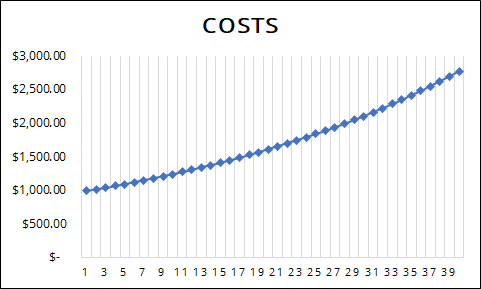
\includegraphics[width=0.6\textwidth]{assets/1534568012402}
	\caption{Nominal cashflow each year for doing nothing (graph)}
	\label{fig:cf-nothing}
\end{figure}

The full detailed calculations can be found in appendix \ref{appendix:nothing}.\\

\subsubsection{Net Present Worth}

The net present value, calculated in excel, using MARR of 3\% is as follows (table \ref{table:npv-nothing}):

\begin{table}[H]
	\centering
	\begin{tabular}{|c|c|}
		\hline
		Period&Nominal NPV\\
		\hline
		5 years&\$4,764.89 in losses\\
 		20 years&\$18,478.41 in losses\\
		40 years&\$35,844.19 in losses\\
		\hline
	\end{tabular}
	\caption{Nominal NPV for the three analyis periods for doing nothing}
	\label{table:npv-nothing}
\end{table}

The full detailed calculations can be found in appendix \ref{appendix:nothing}.\\

\subsubsection{Equivalent Annual Cash Flow}

Given the net present value, we can easily compute the equivalent annual cash flow using Excel's \texttt{PMT} function (table \ref{table:eacf-nothing}):

\begin{table}[H]
	\centering
	\begin{tabular}{|c|c|}
		\hline
		Period   & Nominal EACF           \\
		\hline
		5 years  & \$1,040.44  in losses per year  \\
		20 years & \$1,242.04  in losses per year \\
		40 years & \$1,550.70  in losses per year \\
		\hline
	\end{tabular}
	\caption{Nominal EACF for the three analyis periods for doing nothing}
	\label{table:eacf-nothing}
\end{table}

The full detailed calculations can be found in appendix \ref{appendix:nothing}.\\

\subsection{A - Alternative A}

Recall this alternative implements a small 400 W system. Since this is not enough to replace grid power on any day, we simply have to compute how much energy this system generates in one year first.\\
\\
By taking the weather data from subsection \ref{subsection:weather}, multiply the generation capacity of 400W to the equivalent effective hours of sunlight, we obtain energy in Wh. The energy in Wh for each month is computed and shown in table \ref{table:a-generated} below.

\begin{table}[H]
	\centering
	\begin{tabular}{|l|l l|}
		\hline
		Month & Generated &     \\ \hline
		1     & 13753     & Wh  \\
		2     & 20807     & Wh  \\
		3     & 37818     & Wh  \\
		4     & 65098     & Wh  \\
		5     & 96642     & Wh  \\
		6     & 120434    & Wh  \\
		7     & 125227    & Wh  \\
		8     & 108434    & Wh  \\
		9     & 78117     & Wh  \\
		10    & 47272     & Wh  \\
		11    & 25468     & Wh  \\
		12    & 14982     & Wh  \\ \hline
		Total & 754.05    & kWh \\ \hline
	\end{tabular}
	\caption{Monthly generated solar energy}
	\label{table;a-generated}
\end{table}

Let us start with the 5-year period analysis. In year 0, we establish the initial install cost of \$2,037.98 and the \$360 rebate. As well as the addition to the CCA class 43 account of \$1,018.99 (half of \$2,037.98 by the 1/2 rule).\\
\\
We also set the initial over all solar efficiency to 100\%, expected to decrease at a rate of 0.5\% a year.\\
\\
In year 1, the total total generated energy is 754.05k kWh (base value in year 0) multiplied by the overall panel efficiency of 99.5\% minus the 2\% flat ineffiency due to dust and soil. The total power is therefore 735 kWh this year. Subtracted that from the 8300 kWh usage, we get 7565 kWh drawn from the grid.\\
\\
Taking the energy drawn from the grid and multiplying by that year's electricity rate gives us \$921.40 for the first year. Plus 400W $\times$ \$0.01 per W of Maintenance and opportunity cost per year gives this year's total before-tax cashflow of \$925.40 (real) in losses.\\
\\
This is better than doing nothing, as doing nothing in the year 1 would have costed \$1,010.95 (real). Because of this, we will take the difference (\$1,010.95-\$925.40) as our \textbf{relative benefit} or cost saving. This metric will act as our income to perform tax analysis.\\
\\ 

The relative benefit now is our income and is taxable. Before that, we compute the tax credit from CCA of 30\% of our existing book value. And add the remaining half of the initial cost basis.\\
\\
The taxable income is the relative benefit minus the CCA. If that happens to be less than or equal to 0, we do not have to pay any taxes. However, given our assumption, we also cannot receive payment from the government.\\
\\
The net saved amount (net profit) is the relative benefit minus the tax paid, which would be the corporate tax rate (10\%)\cite{business-tax} multiplied by the taxable income.\\
\\
The same process applies for the following years.\\
\\
In the last year of analyis, year 5. The salvage value, according to the scenario set up above (section \ref{section:scenario}), is just the left over book value in our UCC account, which is \$415.92.\\
\\
This process repeats for analyis period of 20 years as well as 40 years. Except that of spending the replacement costs every 10 years. As such, the UCC account would update with half of the replacement costs added to the account and the next half added the following year.\\
\\
The full cashflow spreadsheet is available in appendix \ref{appendix:a}.

\subsubsection{5 Year Analysis Result}

For an operating life time of 5 years, the nominal NPV savings are -\$978.94 (negative!). That means we're losing almost a thousand dollars if we chose this design option if we're only certain to make use of it for five years. Which is a EUAC of spending \$213.76\\
\\
As expected, the after tax nominal IRR is far below the after tax MARR, at -17.01\%.\\
\\
It would be a blunder to implement this option.\\

\subsubsection{20 Year Analysis Result}

For 20 years, the result is better but still not worthy enough. The nominal NPV in savings are -\$773, or an EUAC of \$168.79. The nominal after tax IRR of the relative benefits is only -2.30\%.\\
\\
Still not far from being a desirable option, due to the lower production of real solar energy, relatively high initial cost, and high cost per watt.\\

\subsubsection{40 Year Analysis Result}

For 40 years, we do eventually make a positive return. The total NPV savings is \$235.40 in 40 years. Which is a saving of EUAB of \$51.40 annually.\\
\\
The nominal after tax IRR for operating for 40 years is 3.67\%, which is above the MARR. Technically, it is desirable to accept this option.\\

\subsubsection{Solar Panel Replacement Analysis}

Solar panel, in this set of analysis, is different from other assets because we did not assume to have a flat replacement rate due to its long lifespan. But given that the efficiency is deteriating at a rate of 0.5\% per year, when is the opportunity cost lost due to the lost efficiencies start becoming a problem?\\
\\
The replacement analysis I have setup sets the defending to be the current solar panels, and we're replacing the defending with the challenger, the exact same model with exact same specifications, except newer.\\
\\
The marginal cost of operating the defender is the opportunity cost of power that did not get generated due to inefficiencies. the lost energy is given by $(1-e_{s_n})\times 754.05\times E_n$ where $e_{s_n}$ is the overall solar efficiency of year $n$, $E_n$ is the electricity rate of year $n$, and 754.05 is the base amount of energy (100\%) in kWh.\\
\\
The marginal cost is always rising because of the constant decrease in efficiency. Therefore we incorporate replacement analysis technique 1: comparing marginal cost to challenger's minimum life cost EUAC.\\
\\
The challenger EUAC is given by the EUAC for operating for $n$ years as lifetime plus the initial cost divided by the lifetime. The excel formula used for this part is \texttt{=PMT(3\%,K91,-NPV(3\%,\$J\$91:J91))+\$C\$15/K91} where 3\% is the MARR, the nested \texttt{PMT} and \texttt{NPV} functions calculate the EUAC for operating the challenger, and C15/K91 is the term that divides the initial install cost by the intended lifetime.\\
\\
In this case, putting the two together, we have the following graph in figure \ref{fig:a-replacement}.\\

\begin{figure}[H]
	\centering
	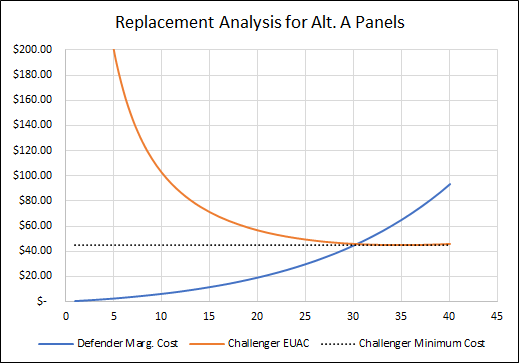
\includegraphics[width=0.75\textwidth]{assets/1534568110958}
	\caption{Replacement analyis (graph) for solar panels in alternative A}
	\label{fig:a-replacement}
\end{figure}

It is clear to see that we need to replace the solar panels at the end of year 28 or 29. But given that our maximum analysis period is only 40 years. The savings in opportunity cost wouldn't break even with the replacement costs given this late into the analysis. Therefore, any replacement of solar panels is illadvised.\\
\\

\subsection{B - Alternative B}

For alternative B, the relative benefits and tax component is identical to that of alternative A's except for the change in design parameter of course.\\
\\
First the solar power generation is different. Because the system has large enough capacity to generate excess energy during summer, we could sell this extra energy. However, at the same time, we don't generate enough power and has to rely on the grid during the winter.\\
\\
The simulation of solar generation and consumption is as follows (table \ref{table:b-generation}).\\
\\
\begin{table}[H]
	\centering
	\begin{tabular}{lllll}
		\hline
		Month & Generated & Consumed & Grid     & Excess   \\
		      & {[}kW{]}  & {[}kW{]} & {[}kW{]} & {[}kW{]} \\ \hline
		1     & 172       & 752      & 580      & 0        \\
		2     & 260       & 726      & 466      & 0        \\
		3     & 473       & 692      & 219      & 0        \\
		4     & 814       & 657      & 0        & 157      \\
		5     & 1208      & 632      & 0        & 576      \\
		6     & 1505      & 623      & 0        & 883      \\
		7     & 1565      & 632      & 0        & 934      \\
		8     & 1355      & 657      & 0        & 698      \\
		9     & 976       & 692      & 0        & 285      \\
		10    & 591       & 726      & 135      & 0        \\
		11    & 318       & 752      & 433      & 0        \\
		12    & 187       & 761      & 574      & 0        \\\hline
		Total & 9426      & 8300     & 2407     & 3533
	\end{tabular}
	\caption{Monthly generated and grid power for alternative B}
	\label{table:b-generation}
\end{table}

It can be seen visually how much energy is pulled from the grid, and how much energy is excess in the summer seasons (figure \ref{fig:b-generation}).\\

\begin{figure}[H]
	\centering
	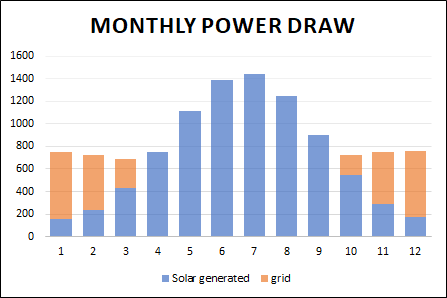
\includegraphics[width=0.55\textwidth]{assets/1534568203596}
	\caption{Monthly generated and grid power for alternative B (graph)}
	\label{fig:b-generation}
\end{figure}

Every year, the excess energy is sold at the buyback rate for that year (starting with 9.99 cents per kWh in 2016). The buyback rate increases annually and is calculated using method outlined in section \ref{subsection:grid}. The full spreadsheet is available in appendix \ref{appendix:grid}.\\
\\
The positive cashflow from selling extra energy contributes to the relative benefits, which is taxable.\\
\\
For analysis B, the payment option is either 5 or 15 years term of loan and no down payment. The listed interest is prime interest rate +2.0\%.\cite{kuby-costs}, which comes out to 5.0\%. To fully repay the loan within the terms, we can use capital recovery factor to determine the annual payment. For 5 years, the annuity is:\\

$$
A=\left(18,620.00\underbrace{-4,500}_\text{rebate}\right)(A/P, 5.0\%, 5)=\$5,571.11
$$

For 15 years:

$$
A=\left(18,620.00\underbrace{-4,500}_\text{rebate}\right)(A/P, 5.0\%, 15)=\$2,323.78 
$$

We integrate this yearly payment for either the first 5 years or 15 years to subtitude the initial payment in year 0.\\
\\
Lastly, we need to consider three separate UCC accounts for our assets because of the assets depreciate at different rates. The set up is straight forward, the costs that associated with each class is added to the account (1/2 applies). The salvage value at the end of the analysis period is the sum of all remaining book values of UCC accounts (see figure \ref{fig:b-cca}).\\

\begin{figure}[H]
	\centering
	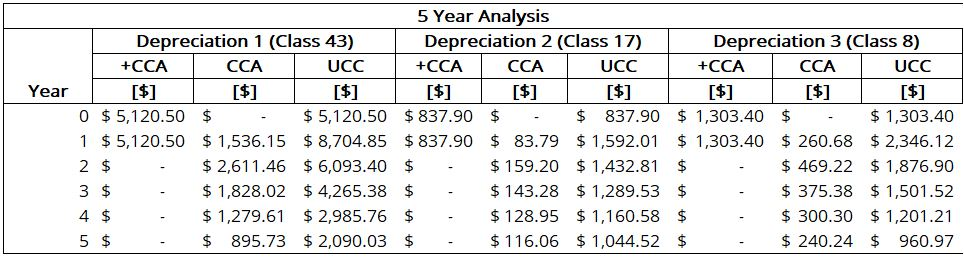
\includegraphics[width=1.0\textwidth]{assets/alternative-b-cca}
	\caption{CCA depreciation on alternative B}
	\label{fig:b-cca}
\end{figure}

The remaining cash flow analyis is identical to that of alternative A. The full spreadsheets can be viewed in appendix \ref{appendix:b}.\\

\subsubsection{5 Year Analyis Result}

For the 5-year analysis period source of capital, there is no option but to choose the 5-year term loan. This means higher annutiy. As a result, and obviously, the project is not worth it:\\
\\
The nominal NPV in savings is -\$6,244.42, or -\$1,363.50 annually as an EUAC. If we look at the cash flow (\ref{appendix:b}), every year, the relative benefit is negative, except when we salvage the assets that's been depreciated for five years already at the end.\\
\\
Overall, because of the short time period, 5 year analyis on larger systems like alternative B or C should never be considered.\\


\subsubsection{20 Year Analyis Result}

For 5 year loan repayment, the nominal IRR for savings is at 1.47\%, below our desired rate. The nominal NPV in savings is -\$1,479.17, or EUAC of -\$322.98.\\
\\
For 15 year loan repayment, the nomianl IRR actually decreases to 0.33\%. The nominal NPV in savings is -\$1,149.96, or EUAC of -\$251.10\\
\\
Nevertheless, both is not recommended. (See full cashflow spreadsheet in appendix \ref{appendix:b}).\\

\subsubsection{40 Year Analysis Result}

With a longer period, the high initial cost is offset by the expensive grid electricity costs in the future.\\
\\
For 5 year loan repayment, the nominal IRR is 5.95\%, far above the desired MARR of 3.0\%! The nominal NPV in savings is \$6,981.29, or EUAB of \$1,524.40.\\
\\
For 15 year loan repayment, the nominal IRR increases to 10.05\%! The nominal NPV in savings is \$7,310.50, or EUAB of \$1,596.28.\\ 

\subsubsection{Solar Panel Replacement Analyis}

The replacement analysis uses the same method as the solar panel replacement analysis for alternative A. Unsurprisingly, because our analysis period is finite and is only 40 years, the replacement year (in figure \ref{fig:b-replacement}) is far too late to make a positive impact.\\

\begin{figure}[H]
	\centering
	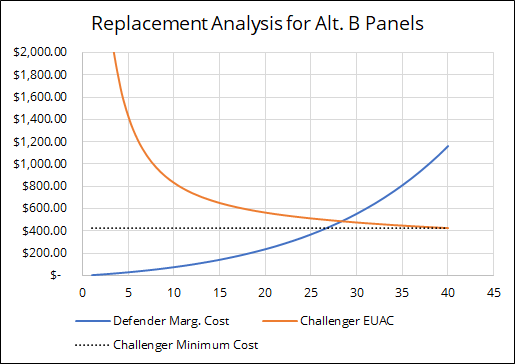
\includegraphics[width=0.6\textwidth]{assets/1534568458573}
	\caption{Replacement analyis for solar panels in alternative B}
	\label{fig:b-replacement}
\end{figure}


\subsection{Alternative C}

The analysis for alternative C is identical to that of alternative B. It is worth noting the solar energy generated. In figure \ref{fig:c-generation}, the increase in solar capacity has shifted the overall generated amount up, thus the grid is less relied during the winter.\\

\begin{figure}[H]
	\centering
	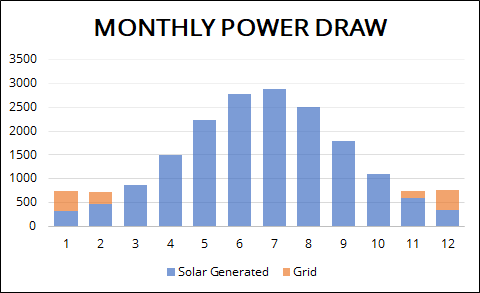
\includegraphics[width=0.6\textwidth]{assets/1534568620011}
	\caption{Monthly generated and grid power for alternative C}
	\label{fig:c-generation}
\end{figure}

\subsubsection{5 Year Analyis Result}

Again, as stated before for alternative B, 5 year is too short given the high initial investment. Using 5 year loan repayment as the only option, the nominal NPV ``savings" are -\$9,667.22. Or EUAC of -\$2,110.88. Not recommended! (See full spreadsheet in appendix \ref{appendix:c}).\\

\subsubsection{20 Year Analyis Result}

With 5 year loan repayment, the nominal IRR for 20 years is 1.81\%, higher that of alternative B's but still not high enough to be worthy of MARR of 3.0\%. The nominal NPV ``savings'' are -\$1,865.47, or EUAC of -\$407.33. (See full spreadsheet in appendix \ref{appendix:c}).\\
\\
With 15 year loan repayment, the nominal IRR decreases to 0.97\%. The nominal NPV ``savings'' are -\$1,299.28, or EUAC of -\$283.70. (See full spreadsheet in appendix \ref{appendix:c}).\\
\\
Both are not recommended once again.\\

\subsubsection{40 Year Analysis Result}\label{subsection:c-40}

Using 5 year loan repayment, the nominal IRR for 40 years is 5.77\%. It is higher than MARR of 3.0\% which is desirable. But it is lower than alternative B's 40 year nominal IRR. Thus further investigation, in particular, incremental IRR analysis is required.\\
\\
Nonetheless, this option has nominal NPV savings of \$10,007.49 and EUAB of \$2,185.18.\\
\\
Using 15 year loan repayment, the nominal IRR is 7.95\%, nominal NPV savings of \$10,573.68 and EUAB of \$2,308.81. (See full spreadsheet in appendix \ref{appendix:c}).\\

\subsubsection{Solar Panel Replacement Analyis}

As shown for alternative A and alternative B, it is not econmical to replace the solar panels themselves, even within a 40 year analysis period. The same applies to alternative C: figure \ref{figure:c-replacement} shows replacement time is 27 years: too late.\\
\\
\begin{figure}[H]
	\centering
	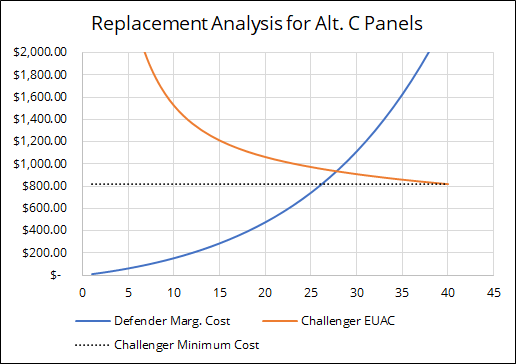
\includegraphics[width=0.6\textwidth]{assets/1534568535020}
	\caption{Replacement analyis for solar panels in alternative C}
	\label{fig:c-replacement}
\end{figure}

\subsubsection{Incremental Rate of Return Analysis}

As stated in section \ref{subsection:c-40}, an incremental rate of return analysis is required to determine which alteranative, B or C, is more profitable.\\
\\
The incremental analysis takes C-B since alternative C is more expensive. For both incremental analysis on 5 or 15 year repayment periods, the incremental IRR is greater than MARR of 3.0\%. Which favors the more expesnive option, alternative C. (See full spreadsheet in appendix \ref{appendix:c}).\\\\
\\

\section{Sensitivity and Risk Analysis}

The biggest risk and source of uncertainty is the weather. According to a study by HeatSpring, author Chris Williams calculated that the weather uncertainty can range between 5\% to 17\%.\cite{solar-production-risk}. Williams' model is for a 35 kW system, his total uncertainty estimate is 12.5\% after weighting everything.\\
\\
This implies that none of our option is worth the risk, at least according to the risk analysis rule of thumb outlined in the course.\\
\\
However, the rule of thumb not always apply to all cases. In this analysis, I tweaked the weather data such that the effective sunlight is 17\% less, the worst case. The result for alternative B and C for the analyis period of 40 years is still above after-tax MARR. Therefore, we can conclude that the system is surprising not sensitive to the sunlight hours. The project viablility still holds. (See appendix \ref{appendix:risk}).\\
\\
The system, however is sensitive to the solar performance efficiency of solar generation. Note that this is not to be confused with the overall solar panel efficiency, which degrades at 0.5\% a year. This is the efficiency that accounts for the solar panel direction to the sun, the effect of sunrise and sunset, etc.\\
\\
At 90\%, the nominal IRR for alternative C, 40 years, is 5.77\%. When the solar performance efficiency increase to 100\% (+10\%) which can be achieved using a tracking device, the nominal IRR increases to 6.65\%. When solar performance is 80\%, the nominal IRR decreases to 4.93\%.\\
\\
This makes sense as the majority of the daylight (50.3\%) is sunlight, and losing 10\% on that is relatively significant to the economic viability of the system.\\
\\

\section{Non-Economic Factors}

Despite the government incentives, Alberta population's main economic driver is still fossil fuel, the public perception and public interst is not as sustainable as we prefer. The low demand from the general public could lead to lower supply of sustainable technlogies such as solar panels which drives up the price.\\
\\
One concern is the safety of the individuals in the household. Eventhough solar panel generation is a rather passive generator, the process of Maintenance could lead to injuries.\\

\section{Conclusion}\label{section:conclusion}

All four alternatives (including doing nothing) cashflow has been analyized to a realitic degree with accurate consumption and weather modelling. The following graph (figure \ref{fig:combined}) shows all four alternatives' net present worth of accmulated total cashflows (not relative benefits).\\

\begin{figure}[H]
	\centering
	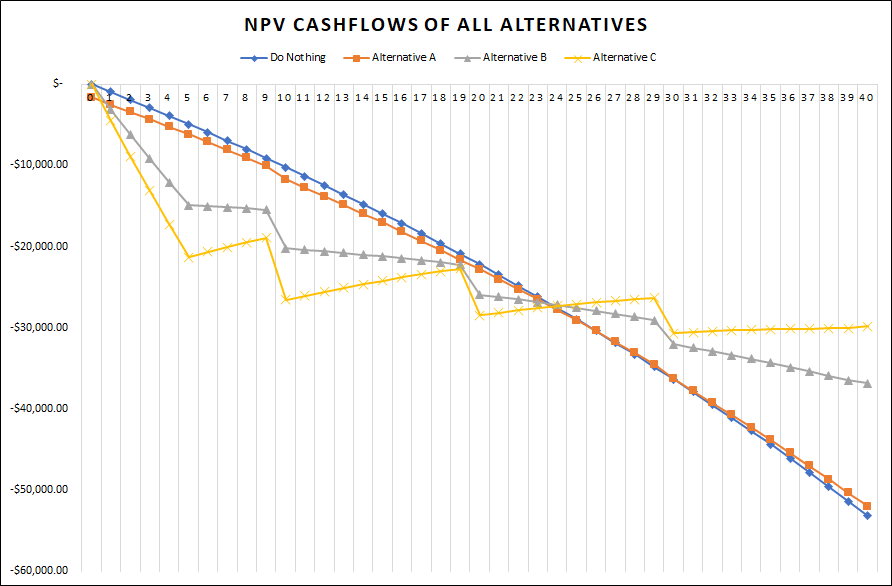
\includegraphics[width=1.0\textwidth]{assets/1534567025903}
	\caption{All alternatives' net present worth cashflows}
	\label{fig:combined}
\end{figure}

The steep slope for alternative B and C at the beginning is due to the repayment of the loans, thus driving the cost higher. Every 10 years, certain parts of the system needs to be replaced, and drops the slope.\\
\\
It is obvious to see that alternative B and C, in the longer term is more benefitial economically. The two options both break-even on year 24. The lighter entry of alternative A is still better than doing nothing, but only breaks-even on year 26. In conclusion, the solar panel is definitely an economic viable project given that it is for certain that it runs for 24 years.\\
\\
Therefore, it is obvious to choose alternative C as it provides the greatest rate of return. Choose 15 year payment over the 5 year payment as this actually offsets the increasing rate of electricity and avoids taxes.\\
\\

% Bibliography
\clearpage
\addcontentsline{toc}{section}{References}
\bibliographystyle{ieeetr}
\bibliography{references}

% Appendix
\clearpage
\appendix
\section{Consumption Calculations}\label{appendix:consumption}
\begin{figure}[H]
	\centering
	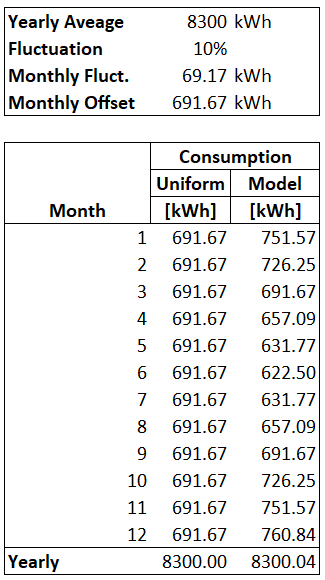
\includegraphics[width=0.3\textwidth]{assets/1534568770072}
	\caption{Spreadsheet calculations on power consumption}
\end{figure}

\clearpage
\section{Weather Calculations}\label{appendix:weather}
\begin{figure}[H]
	\centering
	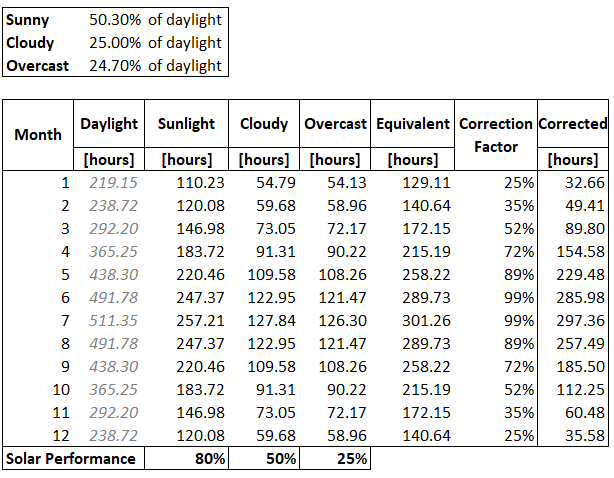
\includegraphics[width=0.7\textwidth]{assets/1534568826258}
	\caption{Spreadsheet calculations on weather model}
\end{figure}

\clearpage
\section{Grid Calculations}\label{appendix:grid}
\begin{figure}[H]
	\centering
	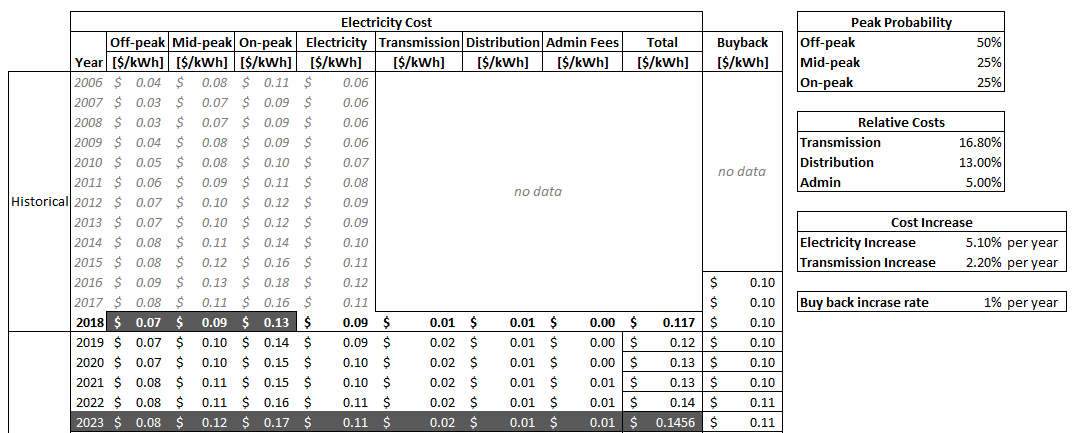
\includegraphics[width=1.0\textwidth]{assets/1534568955354}
	\caption{Spreadsheet calculations on grid electricity model (part 1)}
\end{figure}

\begin{figure}[H]
	\centering
	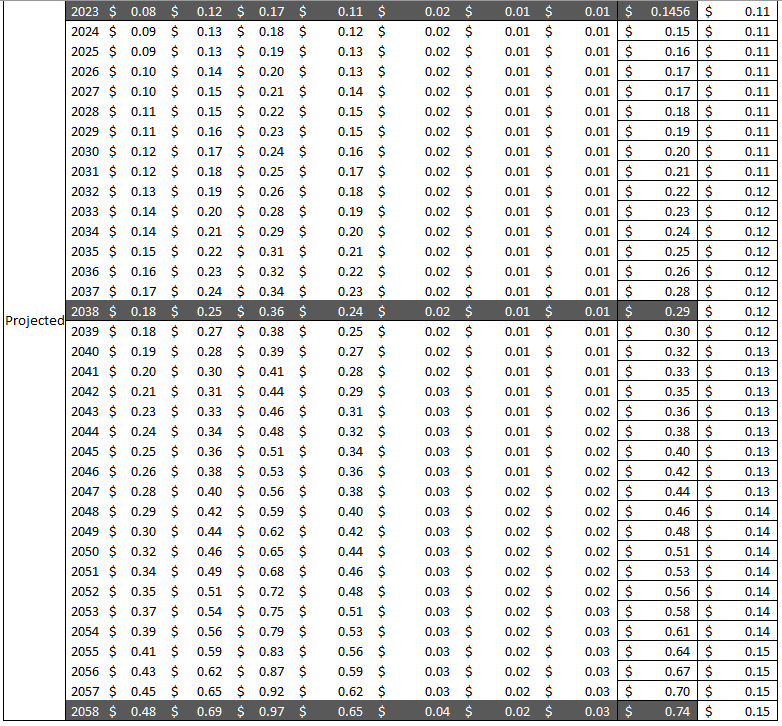
\includegraphics[width=0.7\textwidth]{assets/1534568977509}
	\caption{Spreadsheet calculations on grid electricity model (part 2)}
\end{figure}

\clearpage
\section{Do Nothing Analysis}\label{appendix:nothing}
\begin{figure}[H]
	\centering
	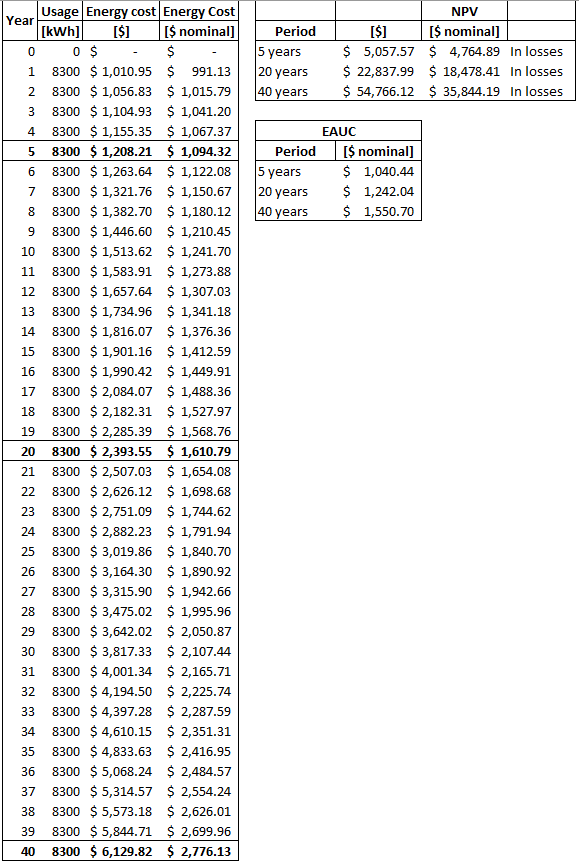
\includegraphics[width=0.75\textwidth]{assets/1534569137295}
	\caption{Spreadsheet cashflow analysis on do nothing option}
\end{figure}

\clearpage
\section{Analysis for Alternative A}\label{appendix:a}
\begin{figure}[H]
	\centering
	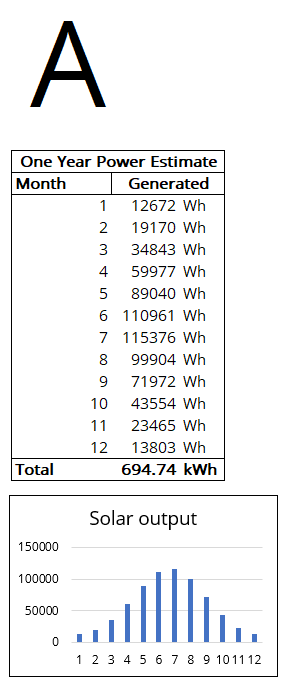
\includegraphics[width=0.3\textwidth]{assets/1534569236076}
	\caption{Spreadsheet cashflow analysis on alternative A (part 1)}
\end{figure}

\begin{figure}[H]
	\centering
	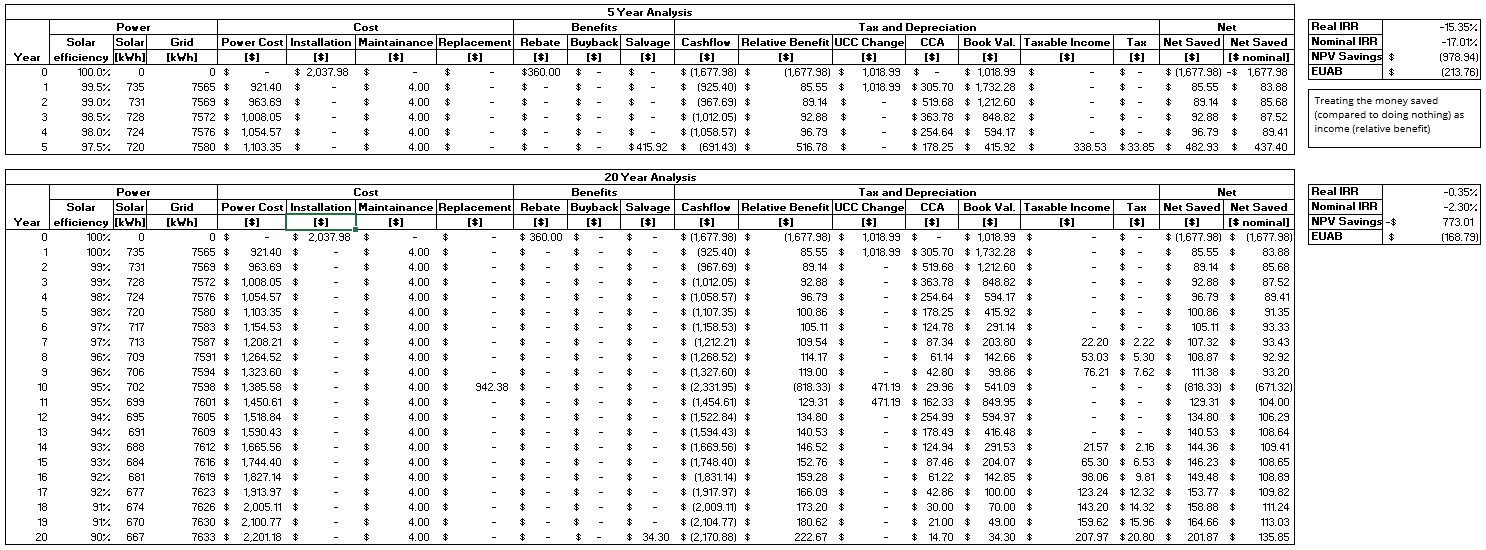
\includegraphics[width=1.0\textwidth]{assets/1534570611392}
	\caption{Spreadsheet cashflow analysis on alternative A (part 2)}
\end{figure}

\begin{figure}[H]
	\centering
	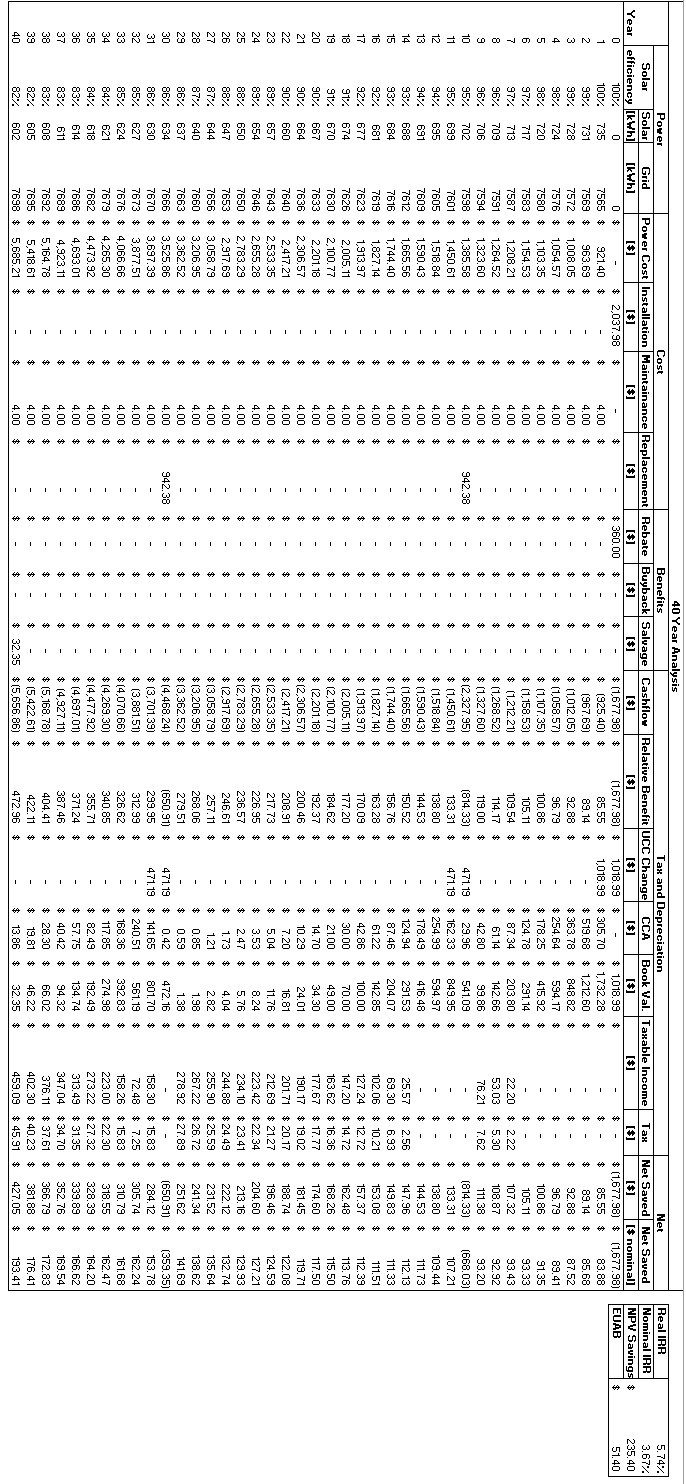
\includegraphics[width=0.5\textwidth]{assets/1534570644880}
	\caption{Spreadsheet cashflow analysis on alternative A (part 3)}
\end{figure}

\begin{figure}[H]
	\centering
	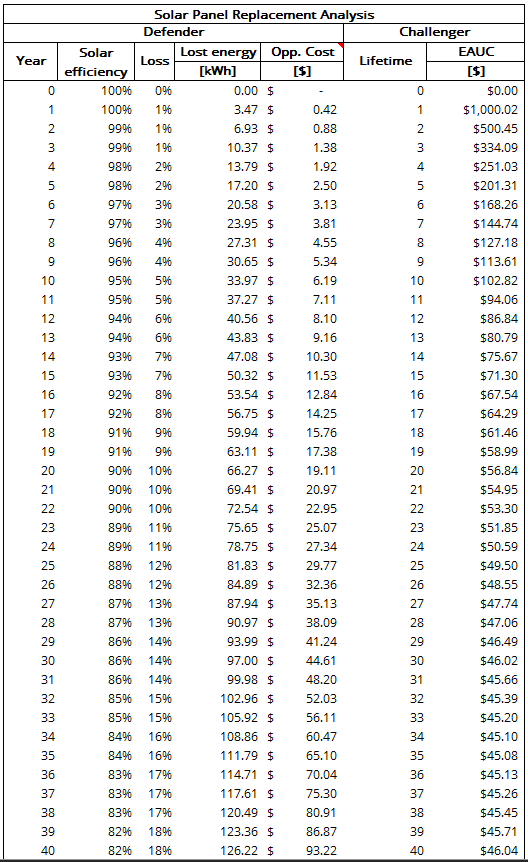
\includegraphics[width=0.5\textwidth]{assets/1534569623916}
	\caption{Spreadsheet cashflow analysis on alternative A (part 4) replacement analysis}
\end{figure}

\clearpage
\section{Analysis for Alternative B}\label{appendix:b}
\begin{figure}[H]
	\centering
	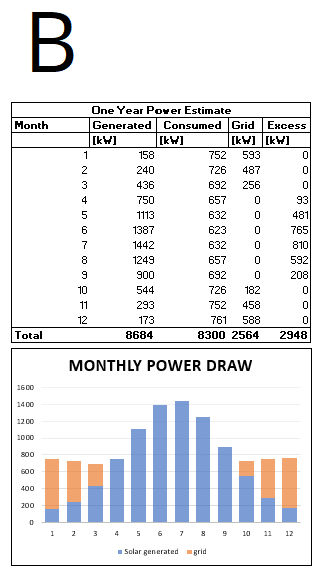
\includegraphics[width=0.3\textwidth]{assets/1534569891414}
	\caption{Spreadsheet cashflow analysis on alternative B (part 1)}
\end{figure}

\begin{figure}[H]
	\centering
	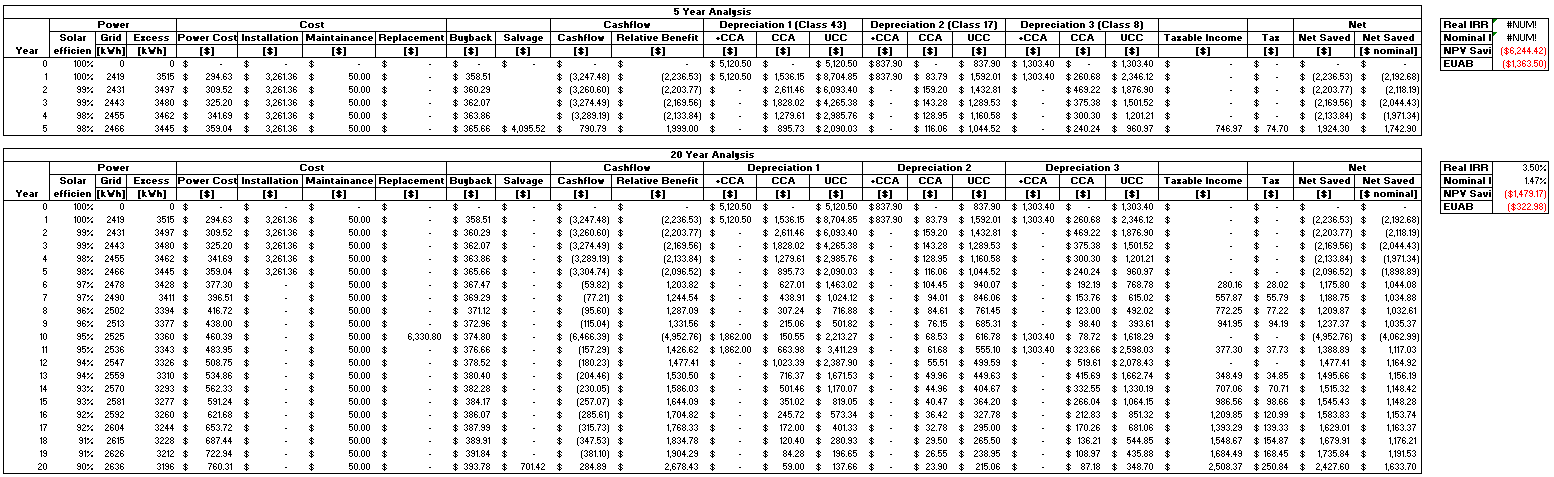
\includegraphics[width=1.0\textwidth]{assets/1534570741142}
	\caption{Spreadsheet cashflow analysis on alternative B (part 2) 5 year repayment}
\end{figure}

\begin{figure}[H]
	\centering
	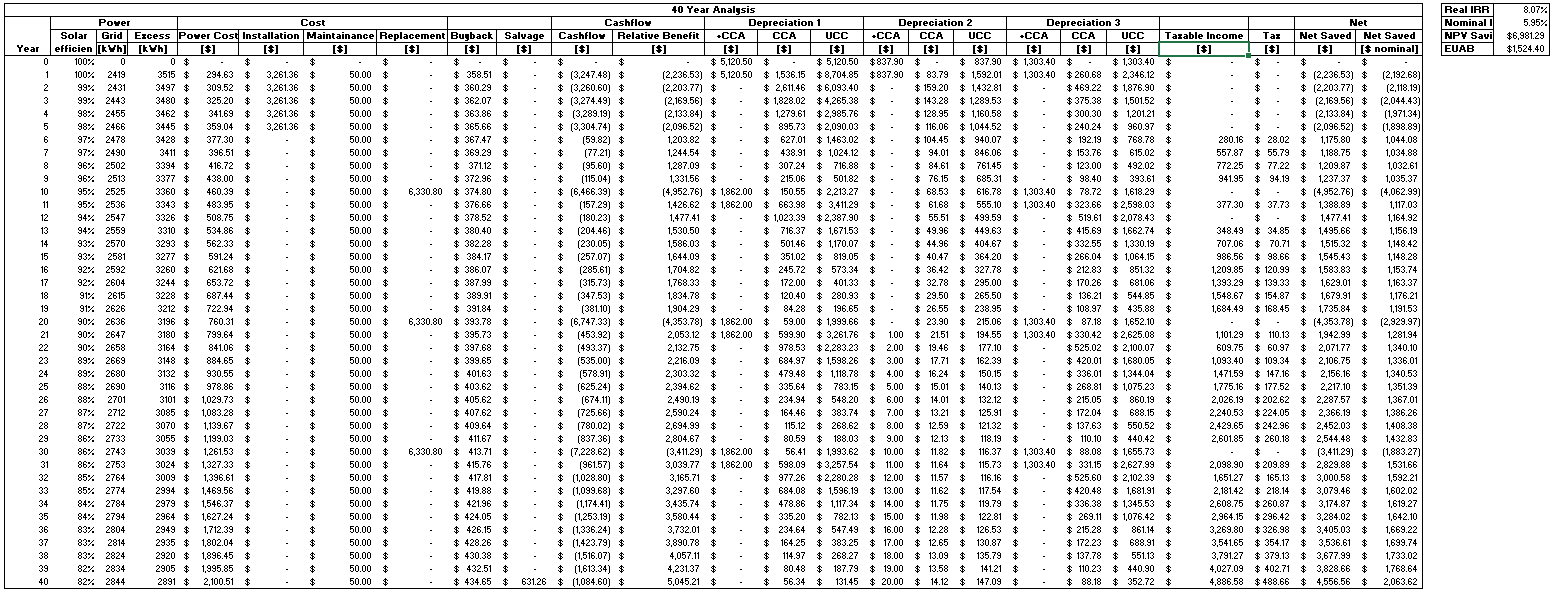
\includegraphics[width=1.0\textwidth]{assets/1534570763068}
	\caption{Spreadsheet cashflow analysis on alternative B (part 3) 5 year repayment}
\end{figure}

\begin{figure}[H]
	\centering
	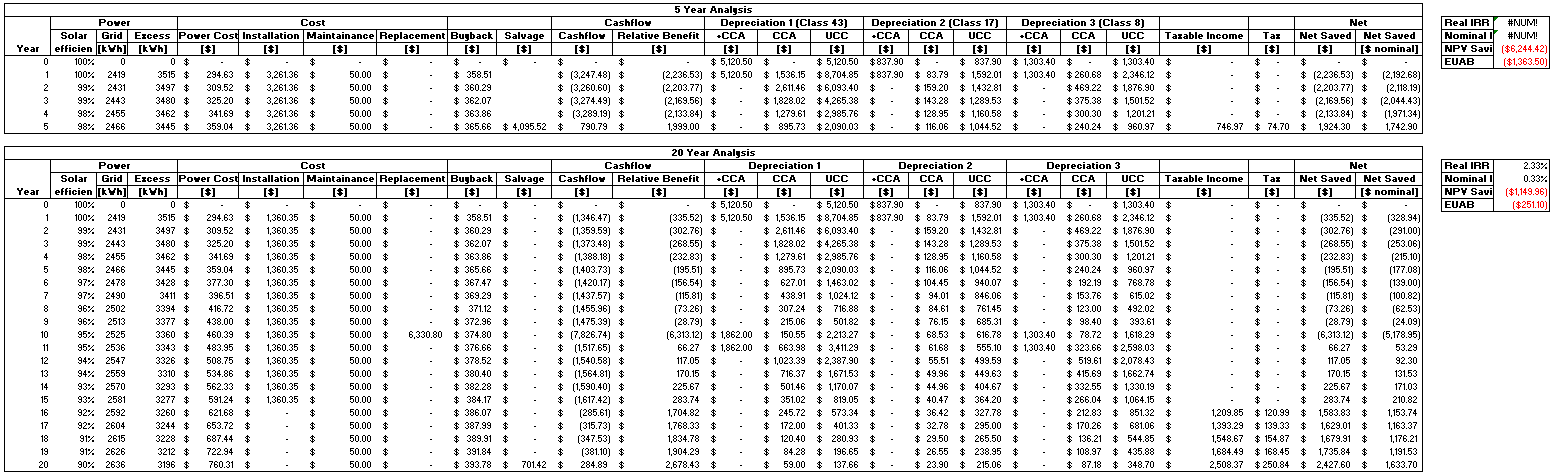
\includegraphics[width=1.0\textwidth]{assets/1534570784889}
	\caption{Spreadsheet cashflow analysis on alternative B (part 4) 15 year repayment}
\end{figure}

\begin{figure}[H]
	\centering
	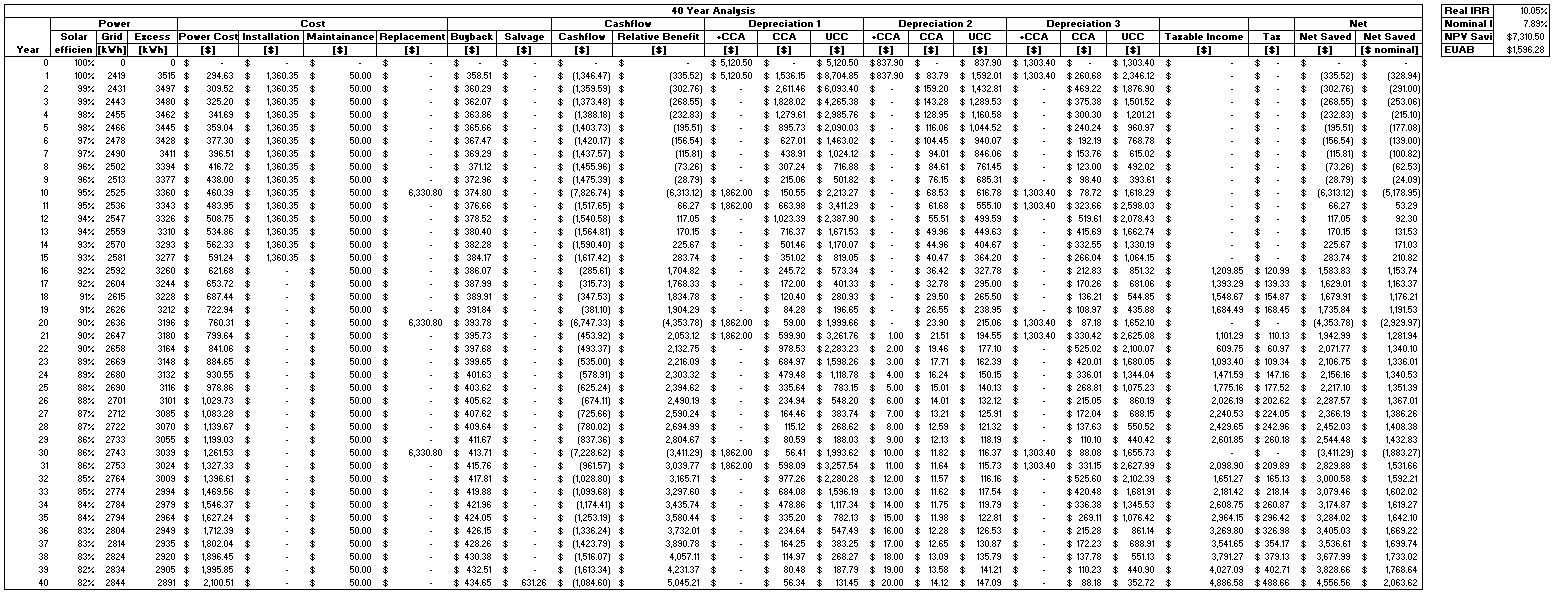
\includegraphics[width=1.0\textwidth]{assets/1534570805126}
	\caption{Spreadsheet cashflow analysis on alternative B (part 5) 15 year repayment}
\end{figure}

\begin{figure}[H]
	\centering
	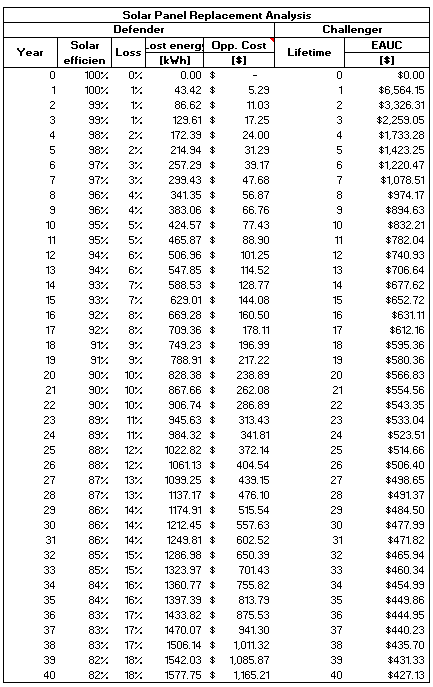
\includegraphics[width=0.5\textwidth]{assets/1534570277965}
	\caption{Spreadsheet cashflow analysis on alternative B (part 5) replacement analysis}
\end{figure}

\clearpage
\section{Analysis for Alternative C}\label{appendix:c}
\begin{figure}[H]
	\centering
	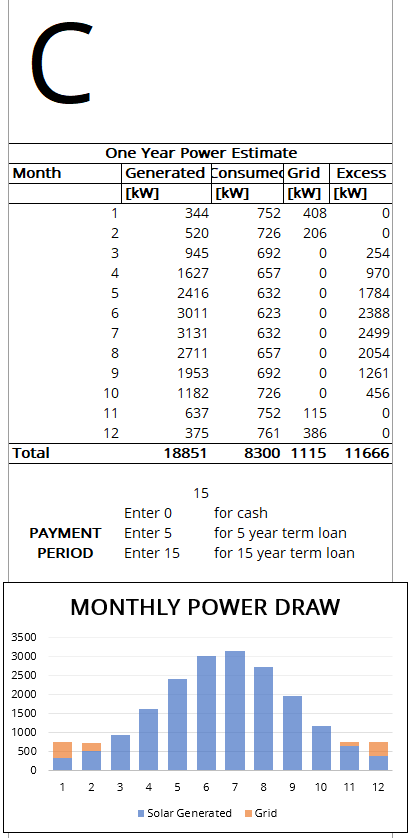
\includegraphics[width=0.3\textwidth]{assets/1534570985625}
	\caption{Spreadsheet cashflow analysis on alternative C (part 1)}
\end{figure}

\begin{figure}[H]
	\centering
	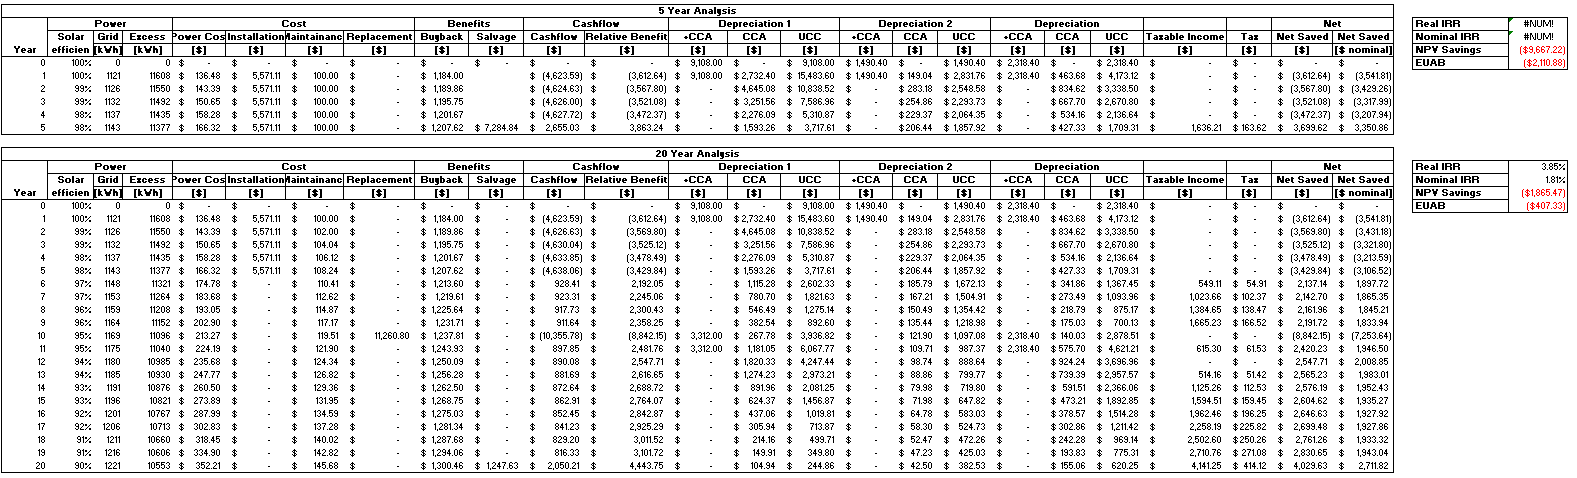
\includegraphics[width=1.0\textwidth]{assets/1534570889581}
	\caption{Spreadsheet cashflow analysis on alternative C (part 2) 5 year repayment}
\end{figure}

\begin{figure}[H]
	\centering
	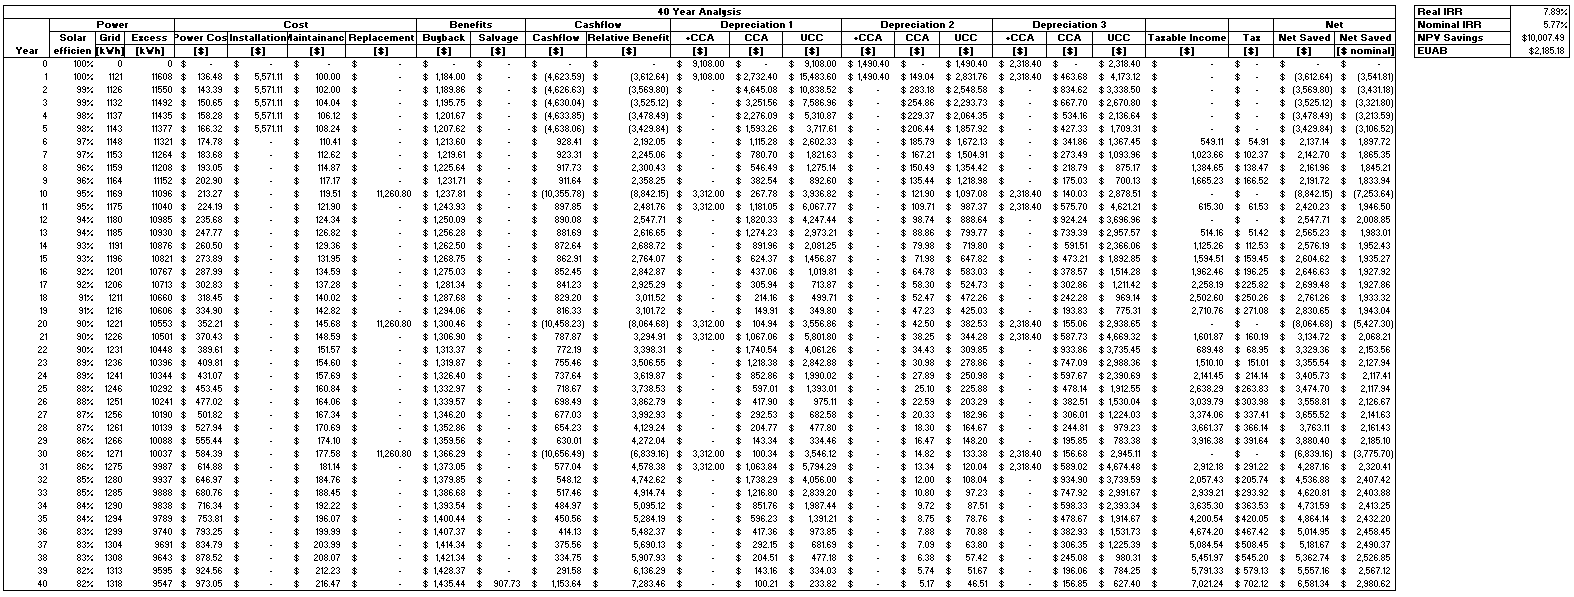
\includegraphics[width=1.0\textwidth]{assets/1534570912032}
	\caption{Spreadsheet cashflow analysis on alternative C (part 3) 5 year repayment}
\end{figure}

\begin{figure}[H]
	\centering
	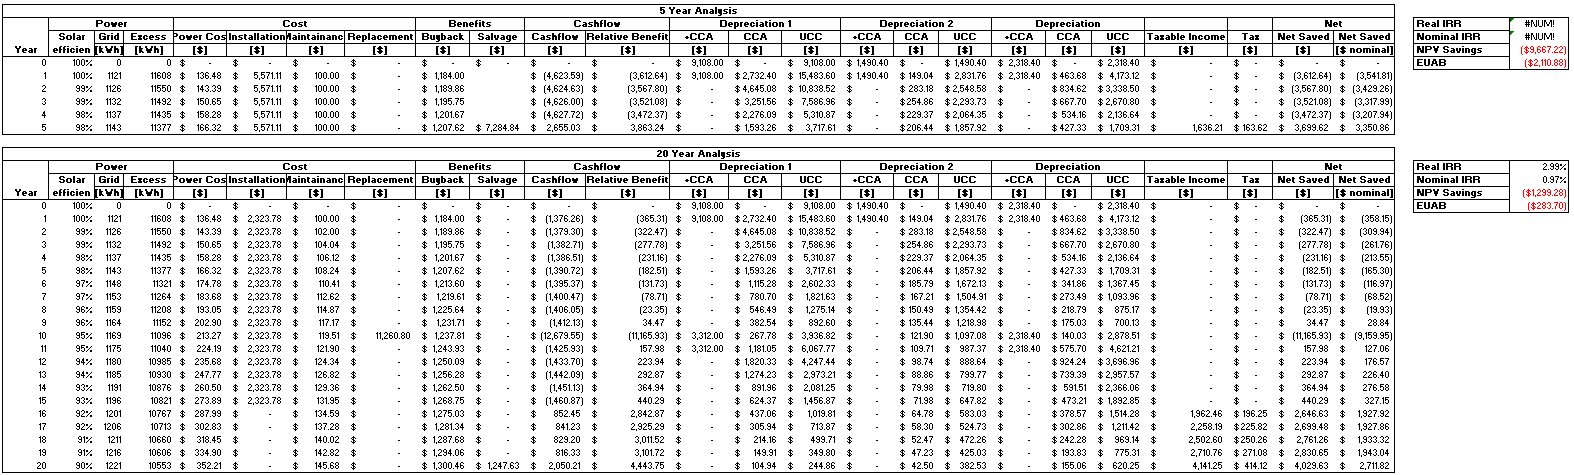
\includegraphics[width=1.0\textwidth]{assets/1534570923844}
	\caption{Spreadsheet cashflow analysis on alternative C (part 4) 15 year repayment}
\end{figure}

\begin{figure}[H]
	\centering
	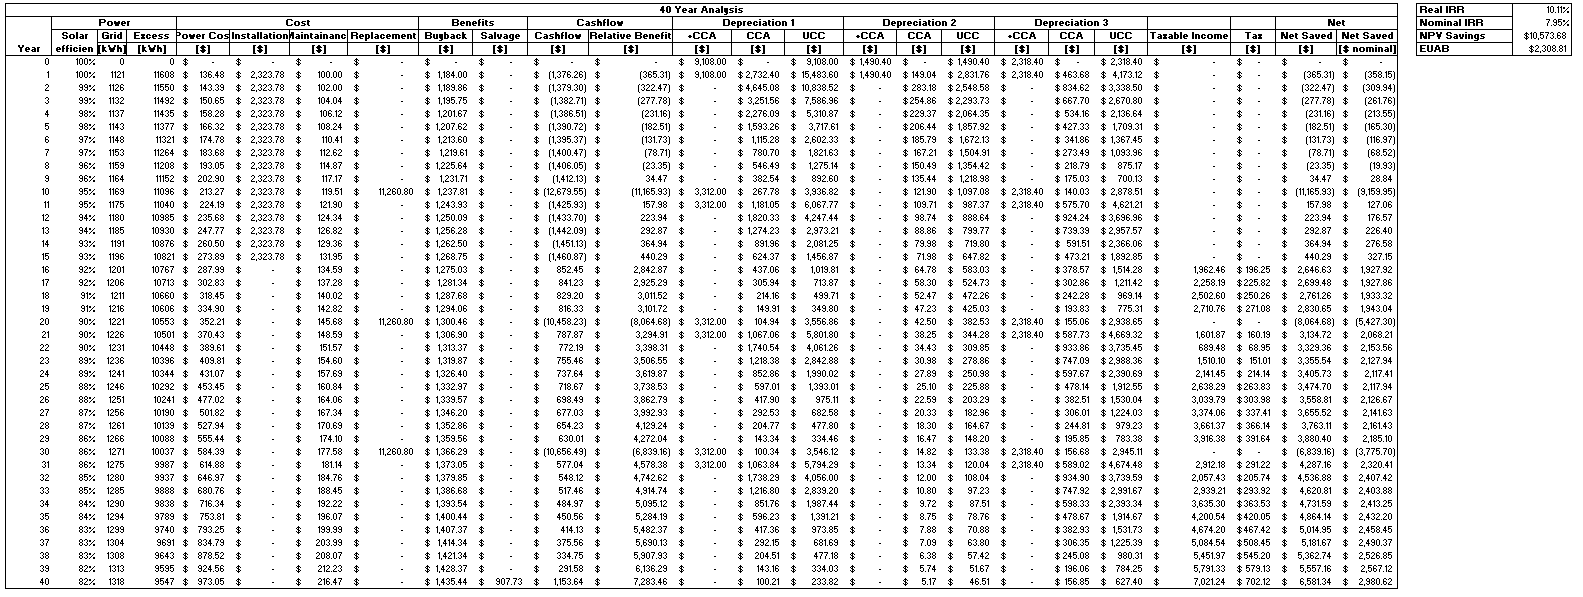
\includegraphics[width=1.0\textwidth]{assets/1534570934621}
	\caption{Spreadsheet cashflow analysis on alternative C (part 5) 15 year repayment}
\end{figure}

\begin{figure}[H]
	\centering
	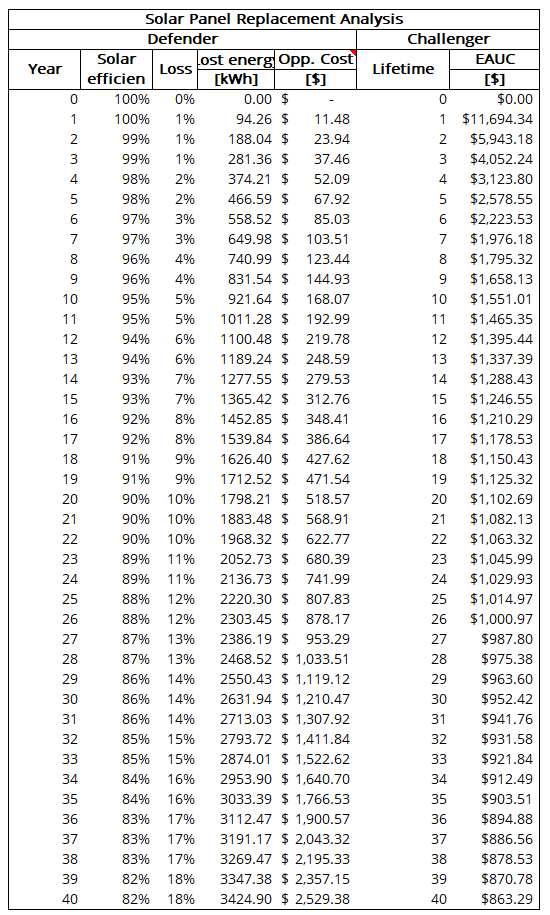
\includegraphics[width=0.5\textwidth]{assets/1534571099518}
	\caption{Spreadsheet cashflow analysis on alternative C (part 6) replacement analysis}
\end{figure}

\begin{figure}[H]
	\centering
	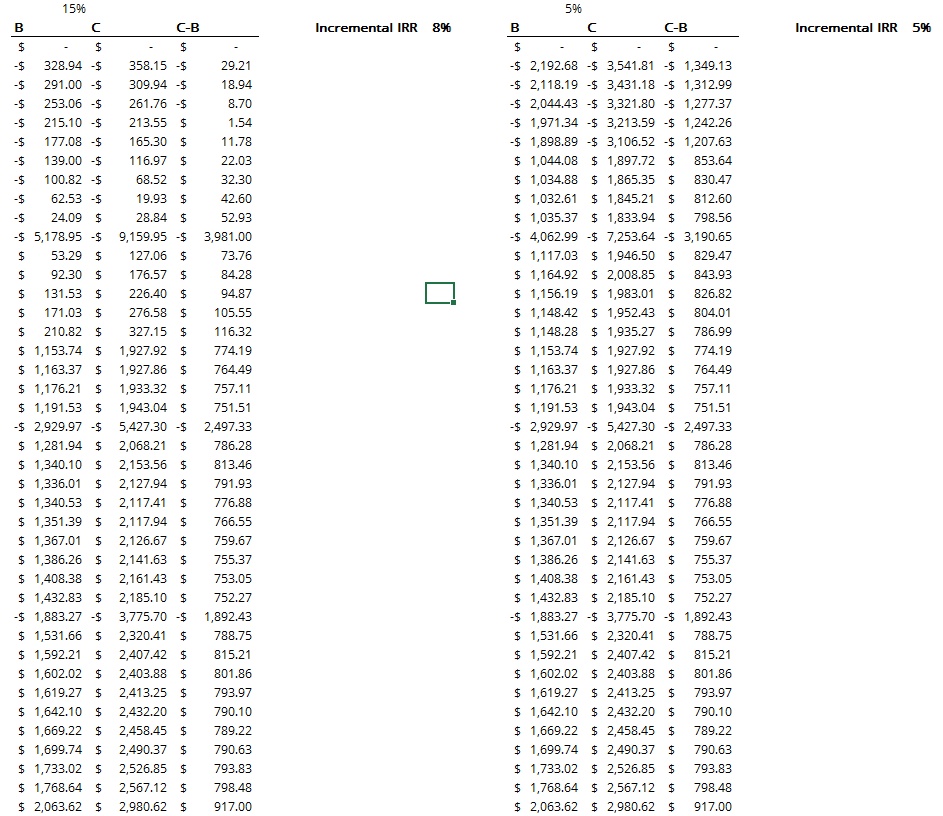
\includegraphics[width=1.0\textwidth]{assets/1534571197467}
	\caption{Spreadsheet cashflow analysis on alternative C (part 7) incremental rate of return analysis}
\end{figure}

\end{document}